\documentclass{article}
\usepackage[review]{log_2026}
\usepackage{booktabs}
\usepackage{multirow}
\usepackage{amsfonts}
\usepackage{graphicx}
\usepackage[numbers,compress,sort]{natbib}

\title[View Selection Limits Multi-Agent Graph Retrieval]{View Selection Limits Multi-Agent Retrieval over Isolated Knowledge Graphs}
\author[Anonymous Authors]{Anonymous Authors}

\begin{document}
\maketitle

\begin{abstract}
Teams reading the same filing under different ontologies and access rules build different graphs, so some questions stay inside one graph while others need several. We built a slot-conditioned router that calls the smallest authorized set of graph specialists able to fill or verify a question's answer slots, and we report what happened when we tried to measure its benefit. Two premises held: isolated category views are measurably different observations once identity is governed, and selective verification is safe under controlled conflict and protected-field stress. The premise that failed is the one we assumed was easy. On 13 blind-validated questions the router finds both required views only four times, and at a fixed 2{,}048-token budget it returns .045 slot recall where uniform random selection at the same coverage already gives .134. Conditioning on the router's own outcome shows why: it beats a term-frequency baseline where selection succeeds (.147 against .083) and scores exactly .000 where it misses, because an uncovered selection serves no evidence at all. A capability fallback repairs the failure at both retrieval and answer level, yet never overtakes simple centralization. We report this as a negative result with the ablations that locate it, because the component the field treats as plumbing is the one that decides whether coalitions of graph agents can work.
\end{abstract}

\section{Introduction}
The same financial filing can support several valid graphs. An accounting team may preserve reporting structure, a risk team may emphasize exposures, and a governance team may record control relationships. Their graphs can disagree about which entity or relation exists even though they read the same document. Merging the views removes the ownership boundary that made each one trustworthy. Keeping them fully separate makes questions that span teams hard to answer.

Graph databases increasingly support multi-tenant and cross-database workloads~\citep{memgraph2026}, which solves the execution problem of letting an authorized application read more than one database. It does not solve the semantic one: which views a question actually needs. Querying every view wastes calls and context, and it can amplify irrelevant or poisoned evidence. Querying one fixed view fails whenever the required evidence is distributed. This is a decision problem before it is a generation problem, and the decision is where we found the difficulty.

Slot-and-Divergence Coalition Routing identifies the facts a question requires, selects the smallest authorized set of category agents that can supply them, and passes only typed evidence to a supervisor. Missing slot coverage and comparable-fact conflict are hard conditions. Graph-divergence statistics only rank candidates that already pass, and Figure~\ref{fig:decision} states the whole rule.

We set out to measure the benefit of that design and found instead that its weakest component is view selection. This extended abstract reports the failure and the two measurements that localize it. Appendix~\ref{app:data} onward carries the full ablation set, the entity-governance and safety results, and the multi-model answer comparison.

\begin{figure}[t]
\centering
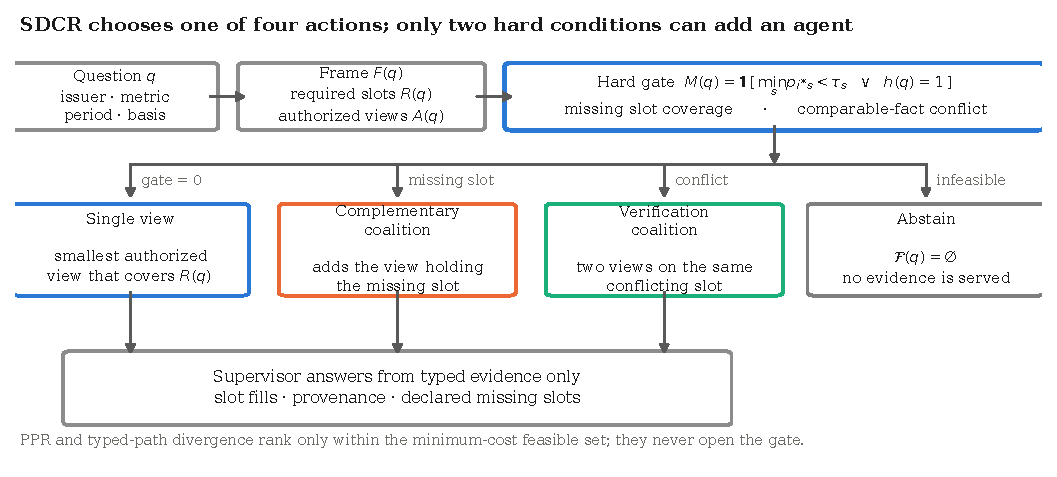
\includegraphics[width=\linewidth]{sdcr_decision.pdf}
\caption{The routing rule. Two hard conditions, a required slot the best single view cannot fill or a comparable-fact conflict, are the only ways an additional agent is called. Divergence statistics rank candidates inside the minimum-cost feasible set and never open the gate. Three of the four actions reach the supervisor; abstention serves no evidence.}
\label{fig:decision}
\end{figure}

\section{Setup}
FinDER contains 5,703 financial questions across eight categories. Four generation models ground every case, yielding 22,812 provider--case workspaces and 523,092 nodes; category views after normalization hold 187,601 semantic nodes, and the qualified answer projection holds 8,313.

Evaluation questions are built without reading any graph output or answer score. A deterministic cap produces 240 cross-view candidates, a provenance gate passes 35, and author screening accepts 28. We then audited that construction blind. Two reviewers from one model family agree on 88.6\% of the candidates but agree with the author on only 77.1\%, and a second panel rejected all nine disputed items because many prompts concatenated two topics without forcing a joint decision. We therefore keep the 28-case result only as a failed exploratory audit. The 28 pairs were rewritten as atomic integrative questions and a five-role blinded gate retained 13 (Appendix~\ref{app:queries}). Persona votes are correlated model simulations and are never labelled human annotation. Candidate-time issuer labels also come from a heuristic rather than a resolved identifier; three of 240 candidates provably pair two different companies, and Appendix~\ref{app:routing} reports the corrected pool.

Retrieval uses compact sorted-key JSON with an exact 2{,}048-token cap under a fixed tokenizer, no truncation of any evidence unit, and the same budget for every arm. Routing and schema failures score zero under intention-to-treat.

\section{The router, not the answerer, is the limiting component}
On the 13 revised questions the frozen slot router selects both required category views in 4 of 13 cases, with mean required-view coverage .538 and 2.54 selected agents. The prompt was not tuned after these labels were seen.

\begin{table}[t]
\centering
\caption{Exact-budget retrieval on the 13 revised cases. Every arm has the same 2,048-token cap and no evidence unit is truncated, so differences reflect view selection and not context size. Slot-only and category-only are, by construction, the frozen term-frequency top-2 and top-1 capability policies.}
\label{tab:retrieval}
\small
\begin{tabular}{lrrr}
\toprule
Arm & Slot token recall & Cross-view recall & Mean tokens\\
\midrule
Qualified-view broadcast (oracle team) & \textbf{.197} & .078 & 1{,}970\\
Centralized single & .184 & .067 & 1{,}974\\
Slot-only $=$ capability top-2 & .132 & .066 & 1{,}985\\
Category-only $=$ capability top-1 & .117 & .057 & 1{,}824\\
Routed SDCR (intention-to-treat) & .045 & .021 & 607\\
\midrule
Uniform random, 2 views (reference) & .066 & .026 & 913\\
\bottomrule
\end{tabular}
\end{table}

Table~\ref{tab:retrieval} and Figure~\ref{fig:bottleneck} make the failure quantitative. Coverage buys recall almost linearly across the random-selection arms, and the oracle team at full coverage reaches .197. The router sits at .538 coverage, above random three-view selection, yet returns .045. The random trend at the same coverage would already deliver .134, a threefold shortfall, and the router also loses outright to a frozen term-frequency capability policy that uses no learned routing at all.

\begin{figure}[t]
\centering
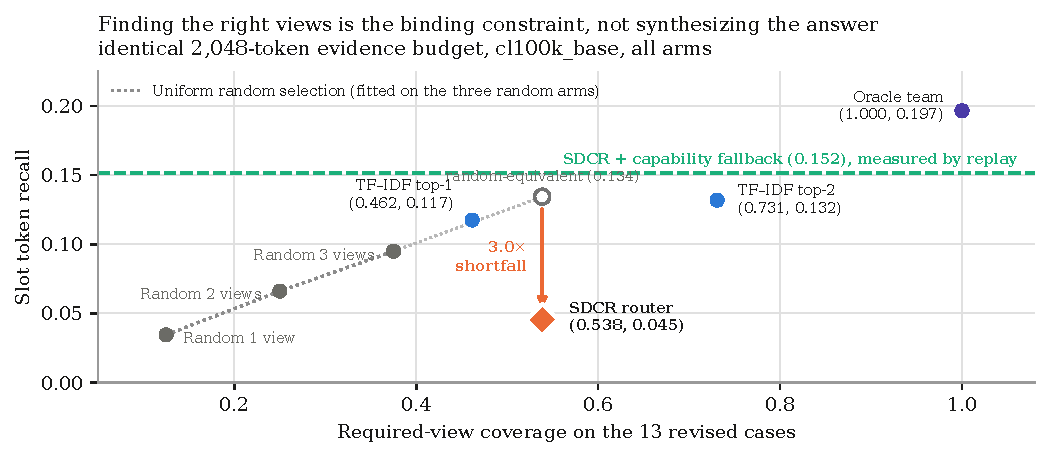
\includegraphics[width=\linewidth]{routing_bottleneck.pdf}
\caption{Required-view coverage against slot token recall at an identical 2,048-token budget. The three uniform-random arms trace what coverage alone is worth. The learned router reaches .538 coverage but .045 recall, a threefold shortfall against the random-equivalent point, and falls below a frozen capability baseline. The gap to the oracle team is the headroom a correct router would recover.}
\label{fig:bottleneck}
\end{figure}

\paragraph{The aggregate comparison hides the actual defect.} Conditioning on the router's own outcome separates two very different behaviors. On the four cases it covers, the routed arm reaches .147 slot recall against .083 for the capability team on those same cases, so where selection succeeds the learned router is the better retriever. On the nine it misses it scores exactly .000, because an uncovered selection serves no evidence, while the capability team reaches .154. The deficit is a failure mode and not weak retrieval.

\paragraph{The repair works, and stops at centralization.} Serving the capability team whenever coverage is incomplete raises retrieval to .152, an increase of .106 with an issuer-clustered 95\% interval of [.052,.164], recovering 77\% of the oracle ceiling instead of 23\% (Appendix~\ref{app:fallback}). Re-answering from that evidence with three models raises slot F1 for all three, and the interval excludes zero for one of them (.067, [.008,.124]). Against centralized single and qualified-view broadcast, however, all six answer intervals contain zero. The repair removes a defect that was masking the comparison; it does not show that coalitions help.

\section{What this does and does not establish}
\label{sec:observation}
Two premises of the design hold, with the supporting tables in Appendix~\ref{app:data} and Appendix~\ref{app:review}. Isolated category views are measurably different observations once identity is governed, separating cross-category from a matched cross-model null with .746 discrimination, and the improvement over a phrase-frequency control has an entity-clustered interval of [.045,.146] that excludes zero. Selective verification is safe under controlled stress: a verification coalition detects 31 of 31 injected conflicts, accepts none of the poisoned values, and filtering the protected field before serialization yields no marker disclosures against 26 of 31 under unsafe broadcast.

A separate calibration gate (Appendix~\ref{app:mediation}) finds that graph-construction changes do not measurably reach answer quality through retrieval. Divergence, by contrast, cannot trigger collaboration. The matched null itself saturates at complete non-overlap, so every empirical upper-tail threshold equals 1.000 and no tested level selects a single cross-category pair. As a tie-break its measured effect is one decision in eighty.

\paragraph{Limitations.} The revised set contains 13 model-constructed and model-validated queries and only four route successfully, so it cannot support a confirmatory answer comparison and we do not offer one. Token overlap remains a lexical measure. The adversarial tests are synthetic and intentionally easy to verify. The candidate-time issuer heuristic must be rebuilt before the wider pool is reused. FinDER categories proxy organizational teams rather than observed ownership and authorization.

\paragraph{Why this is worth reporting.} The field's attention sits on graph construction and on answer synthesis. Our measurements say that with both held fixed, and with the evidence budget held exactly equal, a routing miss that serves nothing costs more than choosing views at random. That is a cheap defect to fix and an expensive one to leave in place, and it is invisible to any evaluation that reports only aggregate answer quality.

\bibliographystyle{plainnat}
\bibliography{references}

\appendix
\section{Reproducibility Protocol}
This appendix specifies the parts of the evaluation that are most vulnerable to hidden supervision or accidental leakage. All procedures write case-level receipts and can be resumed without changing completed calls.

\subsection{FinDER-to-graph construction}
FinDER is a question-and-answer collection rather than a graph dataset. Each record retains a case identifier, financial question, category, issuer or ticker when available, gold answer, and source references. Four generation models read the same source material and emit entity mentions, typed relations, financial values, periods, units, and source links. A provider--case workspace isolates one model's output from another's output.

The extraction pipeline (i) normalizes text while retaining the surface form, (ii) converts model outputs into typed nodes and relations, (iii) normalizes period, unit, and accounting basis while retaining raw values, (iv) keeps duplicate observations until the survivorship policy resolves them, and (v) creates read-only category projections. Every projected fact retains provider, case, category, and source identifiers. The duplicate-aware snapshot contains 22,812 provider--case workspaces, 523,092 nodes, and 1,211,526 relations. Within-category normalization yields 187,601 semantic nodes and 166,147 typed edges; the qualified answer projection contains 8,313 nodes and 20,011 relations.

\begin{table}[h]
\centering
\caption{Complete duplicate-aware category projections.}
\small
\begin{tabular}{lrrrrrrr}
\toprule
View & Nodes & Edges & Degree & LCC & Recip. & Trans. & PR entropy\\
\midrule
Accounting & 17,374 & 13,138 & 1.512 & .501 & .010 & .008 & .991\\
Company overview & 23,399 & 20,326 & 1.737 & .586 & .010 & .009 & .993\\
Financials & 42,978 & 49,758 & 2.316 & .549 & .003 & .009 & .998\\
Footnotes & 58,772 & 37,814 & 1.287 & .438 & .002 & .005 & .998\\
Governance & 12,480 & 11,318 & 1.814 & .503 & .067 & .017 & .982\\
Legal & 14,943 & 12,963 & 1.735 & .553 & .007 & .034 & .993\\
Risk & 7,760 & 10,949 & 2.822 & .673 & .048 & .031 & .973\\
Shareholder return & 9,895 & 6,786 & 1.372 & .434 & .003 & .008 & .996\\
\bottomrule
\end{tabular}
\end{table}
Mean degree measures local connectivity, LCC is the largest-component fraction, reciprocity measures mirrored directed relations, transitivity measures triangle closure, and normalized PageRank entropy measures whether centrality is diffuse. These values describe observation regimes, not category quality. Risk is hub-concentrated despite high connectivity; Footnotes is large but sparse; Governance and Risk have higher reciprocity; Legal has the highest transitivity.

\subsection{Revised-query construction and validation}
Candidate pairs are drawn from the full 5,703-case FinDER pool using issuer, category, and predeclared financial decision axes. Selection does not inspect graphs, retrieval results, answers, or scores. The revision prompt receives only the issuer, two source questions, their gold answers, and the decision axis. It asks for one atomic slot from each view, a conservative cross-view reconciliation, and JSON-only output; unsupported causal claims and simple concatenation are rejected. The initial 28-item construction is retained only as a failed exploratory audit.

Five blinded role/model personas independently validate each revision: financial reporting, audit, equity/benchmark statistics, graph and multi-agent necessity, and governance. An item passes only with at least three of five accepts, valid atomic slots, and a supported cross-view conclusion; the gate issues $28\times5=140$ reviews and retains 13 of 28 items. This five-role revision gate is distinct from the four-persona AGY panel of Appendix~A.4, which examined only the nine disputed or audit-sampled items of the earlier construction. Persona reviews are correlated model simulations and are therefore reported as a robustness audit, not as independent human annotation.

\subsection{Routing and evidence serialization}
Category capability descriptors are deterministic TF--IDF sums over all FinDER questions except component cases in the evaluation item. For token $t$ and $N$ training questions,
\[
 \operatorname{idf}(t)=\log\frac{1+N}{1+\operatorname{df}(t)}+1.
\]
The router selects the smallest authorized coalition satisfying slot coverage. For completeness, the feasible set is
\[
\mathcal{F}(q)=\{C\subseteq A(q):\sum_{i\in C}{\bf 1}[p_{is}\geq\tau_s]\geq r_s(q),\ \forall s\in R(q)\},
\]
where $r_s(q)=2$ only for an explicitly verified or conflicting slot. Personalized PageRank divergence only breaks ties among minimum-cost feasible coalitions; the no-network ablation uses the same candidate set. The revised slot router receives the question and category names, never gold answers or expected categories, and must return a single JSON object. Serialization failures and uncovered required views receive zero in intention-to-treat analysis.

Evidence is compact sorted-key JSON with stable identifiers. Units are appended in retrieval order until the next complete unit would exceed the exact token cap. We use the frozen 
\texttt{cl100k\_base} tokenizer for reproducibility and report sensitivity at 512, 1,024, 2,048, and 4,096 tokens; this does not assert that MARA uses the same tokenizer.

\subsection{Output-blind review and adversarial controls}
The first MARA review is followed by four independent AGY persona critiques and a Codex chair synthesis over the nine disputed or audit-sampled items ($9\times4=36$ reviews per stage). Reviewers do not see author decisions, retrieval outputs, or answer scores. The chair stage is a sensitivity analysis and does not increase the effective reviewer sample size.

For adversarial tests, the query is constructed directly from a matched fact tuple (entity, metric, period, basis, and unit). A poisoned single view receives a 10\% numeric mutation; a verification coalition receives both values and must report a conflict without selecting either. Protected-field tests compare unsafe serialization with SDCR field removal. These 31 answer-blind tests measure contract enforcement under controlled conditions and are not presented as natural-query accuracy.

\subsection{Capability fallback and the corrected candidate pool}
Two artifacts were produced after the main evaluation and are released with it.

The fallback measurement is a replay: the served evidence for each case is assembled from the already-frozen per-case arm rows --- routed evidence where the router covered every required view, the frozen TF--IDF top-2 evidence otherwise --- so retrieval, budget, tokenizer, and provenance are shared exactly with the reported arms and nothing is re-retrieved. The policy was fixed before scores were read. The retrieval half costs nothing and reproduces byte-identically; the answer half re-uses the prompt, schema, and scoring functions of the main harness verbatim, changing only which evidence arm is served, and persists every completion so an interrupted run never repeats a paid call.

The corrected candidate pool re-derives issuer labels with a validated extractor rather than the trailing-acronym heuristic: a token qualifies only as an accepted \texttt{ticker:*} in the frozen identity registry, and a question naming more than one accepted ticker is treated as a cannot-link and dropped. This reuses the identifier-first policy of Section~\ref{sec:observation} instead of introducing a new ticker list. It is released together with a core-disjoint expansion manifest, both marked \texttt{pending\_construct\_validation}; neither contributes to a reported number, because re-deriving the evaluated chain requires re-running the paid five-role gate.

\subsection{Orthogonal mediation gate}
The full corpus has two joint observation profiles and cannot identify prompt and ontology effects separately. We therefore use a mechanistic $2\times2\times4\times16$ calibration: two prompts, two ontologies, four graph-generation models, and 16 FinDER cases. Each cell is read-only, retrieves with the frozen PPR implementation, and is answered by the fixed DeepSeek model. A case-blocked standardized serial path estimates prompt or ontology treatment through graph size and retrieval recall to answer F1. The resulting indirect estimates are reported as calibration evidence, not as full-corpus causal effects.

\section{Results omitted from the main text}
The extended abstract carries only the routing bottleneck. The remaining
measurements are reported here in full so the negative result can be checked
against the evidence that surrounds it.

\subsection{Query-adaptive routing on the synthetic suite}
On an 80-query suite of 28 local, 28 complementary, eight conflict, eight
protected-field, and eight authorization-denied queries, the router behaves well:
it reaches .981 macro F1 at 1.32 mean agent calls. Slot multiplicity and conflict
type supply the signal, since a divergence-only policy is indistinguishable from
centralized routing. Removing the network tie-break changes one of 80 decisions,
raising family accuracy by .0125 with a clustered 95\% interval of $[0,.041]$, so
we claim no detectable network-routing improvement. When one selected specialist
is removed, a capability-level alternative coalition exists in 61.8\% of 34
coalition cases. The contrast with the revised natural questions is the point:
choosing the right \emph{action} is close to solved, while choosing the right
\emph{views} is not. Table~\ref{tab:routing-ea} gives the policy comparison.

\begin{table}[t]
\centering
\caption{Mixed-query routing over 80 queries. Macro F1 and family accuracy measure whether the policy chose the correct action family (local, complementary, verification, or abstain); mean calls measures cost; missed coalition is the fraction of complementary and conflict cases served without the required team. The first three baselines are numerically identical, so they share a row. Every policy except broadcast abstains on all eight unanswerable queries; broadcast never abstains. Broadcast scores zero policy F1 because it has no selective action, even though it retrieves from every view.}
\label{tab:routing-ea}
\small
\begin{tabular}{lrrrr}
\toprule
Policy & Macro F1 & Family acc. & Mean calls & Missed coalition\\
\midrule
Centralized, category-only, divergence-only & .556 & .550 & .90 & 1.000\\
Broadcast & .000 & .000 & 7.90 & 1.000\\
Slot-only & .896 & .863 & 1.21 & .306\\
SDCR, no network & .972 & .963 & 1.31 & .083\\
SDCR & \textbf{.981} & \textbf{.975} & 1.32 & \textbf{.056}\\
\bottomrule
\end{tabular}
\end{table}

\subsection{Multi-model answers}
Substituting the answerer reproduces the deficit instead of removing it. Schema
failure rates are not comparable between the routed and fallback arms, because
routing failures were booked separately from schema violations, so the routed arm
attempted fewer completions. Table~\ref{tab:answers-ea} reports every arm.

\begin{table}[t]
\centering
\caption{Revised 13-case answers under the same 2,048-token cap. Slot F1 measures required fact fields, cross-view F1 the joint reconciliation, and SF the fraction of outputs violating the answer schema. Routing and schema failures receive zero (ITT).}
\label{tab:answers-ea}
\small
\begin{tabular}{llrrrr}
\toprule
Model & Arm & Slot F1 & Numeric recall & Cross-view F1 & SF\\
\midrule
\multirow{4}{*}{DeepSeek-V3.1} & Centralized & .062 & .154 & .123 & .000\\
 & Broadcast & .072 & .108 & .108 & .000\\
 & SDCR & .044 & .031 & .065 & .000\\
 & SDCR $+$ fallback & .071 & .082 & .105 & .000\\
\midrule
\multirow{4}{*}{GPT-OSS-120B} & Centralized & .133 & .284 & .241 & .077\\
 & Broadcast & .128 & .313 & .245 & .077\\
 & SDCR & .038 & .031 & .063 & .000\\
 & SDCR $+$ fallback & .105 & .123 & .207 & .154\\
\midrule
\multirow{4}{*}{MiniMax-M2.7} & Centralized & .012 & .000 & .019 & .923\\
 & Broadcast & .005 & .077 & .013 & .923\\
 & SDCR & .000 & .000 & .000 & .308\\
 & SDCR $+$ fallback & .011 & .000 & .020 & .923\\
\bottomrule
\end{tabular}
\end{table}

\subsection{Orthogonal mediation gate}
A 16-case, 256-cell contrast crossing two prompts, two ontologies, and four
graph-generation models reaches mean retrieval token recall .352 and numeric
recall .886, with a fixed answerer at token overlap .286 and no schema failures.
A case-blocked standardized serial path from treatment through graph size and
retrieval recall to answer quality gives an indirect estimate of $.00006$ for
prompt (95\% interval $[-.00046,.00251]$) and $-.00001$ for ontology
($[-.00099,.00196]$). Graph-construction changes therefore do not measurably
reach answer quality through retrieval in this calibration gate. This is a
mechanistic negative result over two cases per category and not full-corpus
invariance.


\small
\end{document}
